We demonstrate the effectiveness of our approach with the simulation of a
complex manipulation task. In this scenario, two Kuka IIWA arms (7 DOFs each)
are outfitted with anthropomorphic Allegro hands (16 DOFs each), see Fig.
\ref{fig:dual_arm_frames}. In front of the robot, a table has a jar (with a lid,
12 DOFs) full of 16 marbles of $50$~gr each (96 DOFs) and a bowl (6 DOFs), completing the model
with a total of 160 DOFs. Contact between the jar and the lid is modeled using
Drake's hydroelastic model \cite{bib:elandt2019pressure,
bib:masterjohn2021discrete} (see Section \ref{sec:slip_control}), while point
contact is used for all other interactions. The time step is set to $\delta t=5\times 10^{-3}$~s.

The arms' controllers track a prescribed sequence of Cartesian end-effector
keyframe poses, while the hands' controllers track prescribed \emph{open/close}
configurations. We use force feedback to gauge successful grasps and to know
when the jar makes contact with the table. The robot is commanded to open the
jar, pour its contents into the bowl, close the lid and put the empty jar back
in place, see keyframes in Fig. \ref{fig:dual_arm_frames} and the accompanying
video. 

This particular task generates hundreds of contact constraints, as shown in Fig.
\ref{fig:dual_arm_contacts} which also labels important events during the task.

\begin{figure}[!h]
	\centering
    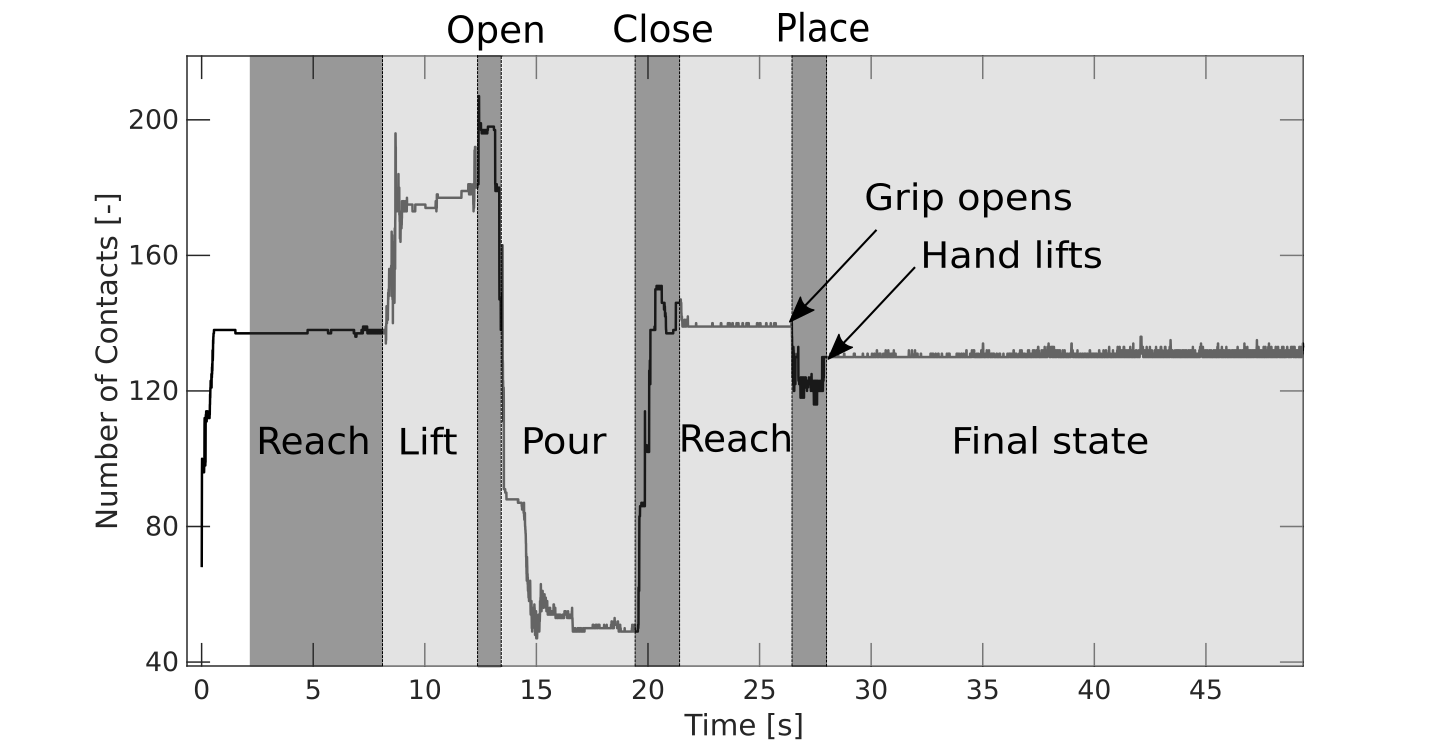
\includegraphics[width=0.9\columnwidth]{figures/dual_arm/dual_arm_contact.png}
    \caption{\label{fig:dual_arm_contacts} Number of contact constraints as a
    function time. Important events during the task are highlighted.}
\end{figure}

To assess accuracy, we evaluate the dimensionless momentum and
complementarity slackness errors defined in Eqs. \eqref{eq:momentum_error} and
\eqref{eq:slackness_error} respectively. We perform the simulation of the same
task several times using different solver tolerances. The results of these runs
are shown in Figures \ref{fig:dual_arm_momentum} and
\ref{fig:dual_arm_slackness}. Even though each solver uses a different tolerance
parameter, it is still useful to place these tolerances in the same horizontal
axis. The maximum tolerance we use for each solver corresponds to the largest value
that can be used to complete the task successfully. For Gurobi and Geodesic IPM,
smaller values of the tolerance parameter make the simulation impractically
slow. SAP on the other hand cannot achieve errors below $10^{-6}$ for this case
due to round-off errors. Figures \ref{fig:dual_arm_momentum} and
\ref{fig:dual_arm_slackness} show both mean and median of the errors over the
entire simulation to show errors do not follow a symmetric distribution. More
interesting however are the minimum and maximum errors, shown as shaded areas.
SAP guarantees that momentum errors are below the specified tolerance, given
this is precisely its stopping criteria in Eq. \eqref{eq:stopping_criteria}. We
see however that it is difficult to correlate the expected error to solver
tolerance when using Gurobi or Geodesic IPM. In practice, we consistently
observed that the simulation did not complete the task successfully when
momentum errors were larger than about $10\%$, regardless of the solver.
Therefore, we found that being able to specify a tolerance for the momentum
error directly is immensely useful. Given that SAP satisfies the complementarity
slackness condition exactly, complementarity slackness error for SAP is not
included in Fig. \ref{fig:dual_arm_slackness}.

\begin{figure}[!h]
	\centering
    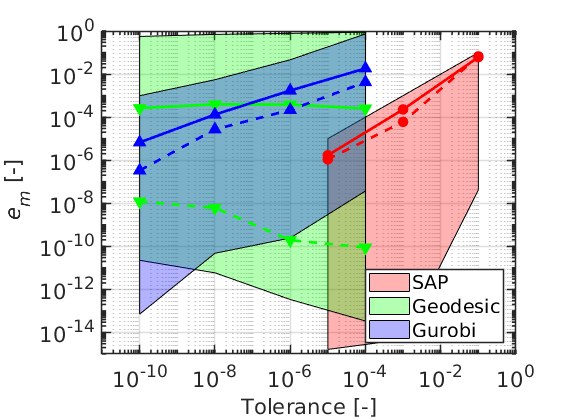
\includegraphics[width=0.7\columnwidth]{figures/dual_arm/momentum_error.png}
    \caption{\label{fig:dual_arm_momentum} Dimensionless momentum error, defined
    in Eq. \eqref{eq:momentum_error}. Mean (solid) and median (dashed) errors
    along with minimum and maximum errors (shaded areas) over the entire simulation.}
\end{figure}

\begin{figure}[!h]
	\centering
    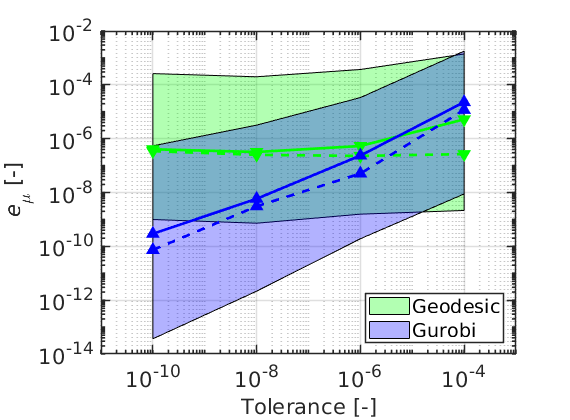
\includegraphics[width=0.7\columnwidth]{figures/dual_arm/optimality_condition.png}
    \caption{\label{fig:dual_arm_slackness} Dimensionless complementarity
    slackness error, defined in Eq. \eqref{eq:slackness_error}. Mean (solid) and
    median (dashed) errors along with minimum and maximum errors (shaded areas) over
    the entire simulation.}
\end{figure}

Figure \ref{fig:dual_arm_iterations} shows the mean number of iterations per
time-step for each solver. We see that the number of iterations needed by the
SAP solver is consistently below the other two solvers given how effectively SAP
warm-starts from the previous time-step solution.

To make a fair comparison among solvers, from Fig.
\ref{fig:dual_arm_momentum} we choose tolerances for each solver that result in
similar values of the mean momentum error. For Gurobi we set its tolerance
parameter \verb+BarQCPConvTol+ to $10^{-8}$, for Geodesic IPM, we set its
complementary slackness tolerance to $10^{-6}$ and for SAP its relative tolerance is set
to $10^{-3}$. Notice this is not entirely fair to SAP, given that SAP does
guarantee the maximum momentum error to be below $10^{-3}$, while this is not
true for the other two solvers. Still, SAP is 7.4 faster than Gurobi and 2.2
faster than Geodesic IPM. In terms of iterations, SAP performs 4 iterations on
average while Geodesic IPM performs 8.3 iterations on average. This shows that
since both solvers use exactly the same sparse algebra, the performance gains
with SAP are entirely due to its ability to warm-start effectively rather than
to differences in the implementation. The general purpose solver Gurobi on the
other hand performs 10.1 iterations on average.

\begin{figure}[!h]
	\centering
    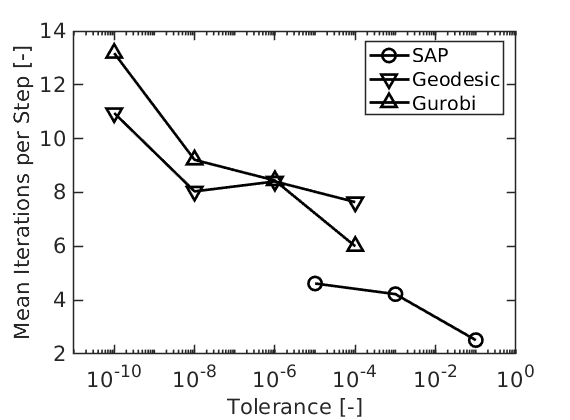
\includegraphics[width=0.7\columnwidth]{figures/dual_arm/iterations_per_step.png}
    \caption{\label{fig:dual_arm_iterations} Mean number of iterations per
    time-step for the dual arm simulation.}
\end{figure}

In summary, the simulation of this complex robotic task demonstrates how
accuracy translates directly to robustness. We observed how the maximum momentum
error defined in Eq. \eqref{eq:momentum_error} is a good proxy for robustness in
simulation; simulations with errors larger than about $10\%$ could not complete
the task successfully. In this regard SAP provides a certificate of accuracy
that proves useful in practice.

